\documentclass[12pt]{article}
\usepackage{tikz}
\usepackage{amsmath}
% Underlining package
\usepackage{ulem}
\usetikzlibrary{calc}
\usepackage[a4paper, portrait, margin=1cm]{geometry}
\usepackage{fancyhdr}

\def \HeadingQuestions {\section*{\Large Name: \underline{\hspace{8cm}} \hfill Date: \underline{\hspace{3cm}}} \vspace{-3mm}
{Angles in a Triangle: Questions} \vspace{1pt}\hrule}

% raise footer with page number; no header
\fancypagestyle{myfancypagestyle}{
  \fancyhf{}% clear all header and footer fields
  \renewcommand{\headrulewidth}{0pt} % no rule under header
  \fancyfoot[C] {\thepage} \setlength{\footskip}{14.5pt} % raise page number allowed min 14.5pt
}
\pagestyle{myfancypagestyle}  % apply myfancypagestyle

\newcounter{minipagecount}

\begin{document}
\HeadingQuestions
\vspace{8mm}

\begin{minipage}{0.55\textwidth}
  \refstepcounter{minipagecount}
  \noindent{(\theminipagecount)}\quad
  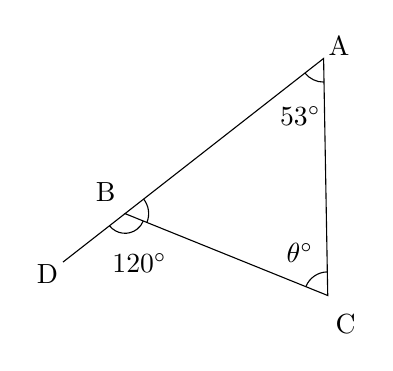
\begin{tikzpicture}[scale=1.0, baseline=(current bounding box.north)]

      \begin{scope}[rotate=218]
        \coordinate (A) at (0,0);
        \coordinate (B) at (3.2003071392851323,0);
        \coordinate (D) at (4.200307139285132,0);
        \coordinate (C) at (intersection cs: first line={(A)--($(A)+(53:4cm)$)}, second line={(B)--($(B)+(180-60:4cm)$)});
        \draw (A) -- (B) -- (C) -- cycle;
        \draw (B) -- (D);

        % Mark angles with arcs
        \draw ($(A)!0.3cm!(B)$) arc [start angle=0, end angle=53, radius=0.3cm];
        \draw ($(B)!0.3cm!(C)$) arc [start angle=180-60, end angle=180, radius=0.3cm];
        \draw ($(C)!0.3cm!(A)$) arc [start angle=180+53, end angle=360-60, radius=0.3cm];
        \draw ($(B)!0.25cm!(D)$) arc [start angle=0, end angle=180-60, radius=0.25cm];

        % Label angles
        \node at ($(A)!-0.25cm!(B)$) {A};
        \node at ($(B)!-0.45cm!(C)!0.2cm!(A)$) {B};
        \node at ($(C)!-0.25cm!(A)!-0.25cm!(B)$) {C};
        \node at ($(D)!-0.25cm!(A)$) {D};

        % Mark angles in degrees
        \coordinate (midBC) at ($(B)!0.5!(C)$);
        \node at ($(A)!0.70cm!(midBC)!0.10cm!(C)$) {$53^\circ$};

        \coordinate (midAC) at ($(A)!0.5!(C)$);
        \node at ($(B)!0.65cm!(midAC)$) {};

        \coordinate (midAB) at ($(A)!0.5!(B)$);
        \node at ($(C)!0.65cm!(midAB)$) {$\theta^\circ$};

        \coordinate (midDC) at ($(D)!0.3!(C)$);
        \node at ($(B)!0.65cm!(midDC)$) {$120^\circ$};


      \end{scope}
    \end{tikzpicture}
\end{minipage}%
\hfill
\begin{minipage}{0.4\textwidth}
  \begin{align*}
    \angle \text{C} &= \angle \text{\dotuline{~~~~~~~}} - \angle \text{\dotuline{~~~~~~~}} \\
    &= \dotuline{~~~~~~~}^\circ  - \dotuline{~~~~~~~}^\circ \\
    &= \dotuline{~~~~~~~}^\circ
  \end{align*}
\end{minipage}
\vspace{1cm} \vfill\begin{minipage}{0.55\textwidth}
  \refstepcounter{minipagecount}
  \noindent{(\theminipagecount)}\quad
  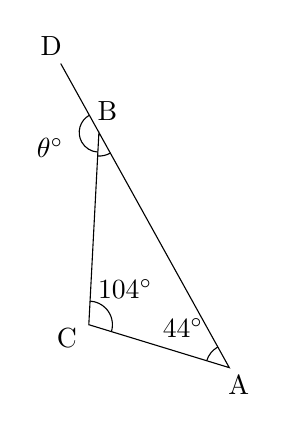
\begin{tikzpicture}[scale=1.0, baseline=(current bounding box.north)]

      \begin{scope}[rotate=119]
        \coordinate (A) at (0,0);
        \coordinate (B) at (3.415352531556346,0);
        \coordinate (D) at (4.415352531556346,0);
        \coordinate (C) at (intersection cs: first line={(A)--($(A)+(44:4cm)$)}, second line={(B)--($(B)+(180-32:4cm)$)});
        \draw (A) -- (B) -- (C) -- cycle;
        \draw (B) -- (D);

        % Mark angles with arcs
        \draw ($(A)!0.3cm!(B)$) arc [start angle=0, end angle=44, radius=0.3cm];
        \draw ($(B)!0.3cm!(C)$) arc [start angle=180-32, end angle=180, radius=0.3cm];
        \draw ($(C)!0.3cm!(A)$) arc [start angle=180+44, end angle=360-32, radius=0.3cm];
        \draw ($(B)!0.25cm!(D)$) arc [start angle=0, end angle=180-32, radius=0.25cm];

        % Label angles
        \node at ($(A)!-0.25cm!(B)$) {A};
        \node at ($(B)!-0.45cm!(C)!0.2cm!(A)$) {B};
        \node at ($(C)!-0.25cm!(A)!-0.25cm!(B)$) {C};
        \node at ($(D)!-0.25cm!(A)$) {D};

        % Mark angles in degrees
        \coordinate (midBC) at ($(B)!0.5!(C)$);
        \node at ($(A)!0.70cm!(midBC)!0.10cm!(C)$) {$44^\circ$};

        \coordinate (midAC) at ($(A)!0.5!(C)$);
        \node at ($(B)!0.65cm!(midAC)$) {};

        \coordinate (midAB) at ($(A)!0.5!(B)$);
        \node at ($(C)!0.65cm!(midAB)$) {$104^\circ$};

        \coordinate (midDC) at ($(D)!0.3!(C)$);
        \node at ($(B)!0.65cm!(midDC)$) {$\theta^\circ$};


      \end{scope}
    \end{tikzpicture}
\end{minipage}%
\hfill
\begin{minipage}{0.4\textwidth}
  \begin{align*}
    \angle \text{DBC} &= \angle \text{\dotuline{~~~~~~~}} + \angle \text{\dotuline{~~~~~~~}} \\
    &= \dotuline{~~~~~~~}^\circ  + \dotuline{~~~~~~~}^\circ \\
    &= \dotuline{~~~~~~~}^\circ
  \end{align*}
\end{minipage}
\vspace{1cm} \vfill\begin{minipage}{0.55\textwidth}
  \refstepcounter{minipagecount}
  \noindent{(\theminipagecount)}\quad
  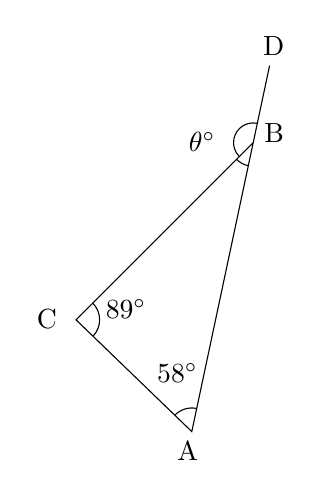
\begin{tikzpicture}[scale=1.0, baseline=(current bounding box.north)]

      \begin{scope}[rotate=78]
        \coordinate (A) at (0,0);
        \coordinate (B) at (3.7519885612751125,0);
        \coordinate (D) at (4.7519885612751125,0);
        \coordinate (C) at (intersection cs: first line={(A)--($(A)+(58:4cm)$)}, second line={(B)--($(B)+(180-33:4cm)$)});
        \draw (A) -- (B) -- (C) -- cycle;
        \draw (B) -- (D);

        % Mark angles with arcs
        \draw ($(A)!0.3cm!(B)$) arc [start angle=0, end angle=58, radius=0.3cm];
        \draw ($(B)!0.3cm!(C)$) arc [start angle=180-33, end angle=180, radius=0.3cm];
        \draw ($(C)!0.3cm!(A)$) arc [start angle=180+58, end angle=360-33, radius=0.3cm];
        \draw ($(B)!0.25cm!(D)$) arc [start angle=0, end angle=180-33, radius=0.25cm];

        % Label angles
        \node at ($(A)!-0.25cm!(B)$) {A};
        \node at ($(B)!-0.45cm!(C)!0.2cm!(A)$) {B};
        \node at ($(C)!-0.25cm!(A)!-0.25cm!(B)$) {C};
        \node at ($(D)!-0.25cm!(A)$) {D};

        % Mark angles in degrees
        \coordinate (midBC) at ($(B)!0.5!(C)$);
        \node at ($(A)!0.70cm!(midBC)!0.10cm!(C)$) {$58^\circ$};

        \coordinate (midAC) at ($(A)!0.5!(C)$);
        \node at ($(B)!0.65cm!(midAC)$) {};

        \coordinate (midAB) at ($(A)!0.5!(B)$);
        \node at ($(C)!0.65cm!(midAB)$) {$89^\circ$};

        \coordinate (midDC) at ($(D)!0.3!(C)$);
        \node at ($(B)!0.65cm!(midDC)$) {$\theta^\circ$};


      \end{scope}
    \end{tikzpicture}
\end{minipage}%
\hfill
\begin{minipage}{0.4\textwidth}
  \begin{align*}
    \angle \text{DBC} &= \angle \text{\dotuline{~~~~~~~}} + \angle \text{\dotuline{~~~~~~~}} \\
    &= \dotuline{~~~~~~~}^\circ  + \dotuline{~~~~~~~}^\circ \\
    &= \dotuline{~~~~~~~}^\circ
  \end{align*}
\end{minipage}
\vspace{1cm} \vfill\begin{minipage}{0.55\textwidth}
  \refstepcounter{minipagecount}
  \noindent{(\theminipagecount)}\quad
  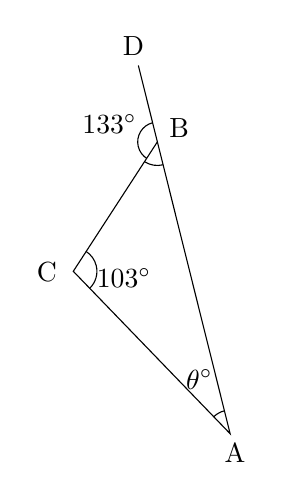
\begin{tikzpicture}[scale=1.0, baseline=(current bounding box.north)]

      \begin{scope}[rotate=104]
        \coordinate (A) at (0,0);
        \coordinate (B) at (3.820050873625135,0);
        \coordinate (D) at (4.820050873625135,0);
        \coordinate (C) at (intersection cs: first line={(A)--($(A)+(30:4cm)$)}, second line={(B)--($(B)+(180-47:4cm)$)});
        \draw (A) -- (B) -- (C) -- cycle;
        \draw (B) -- (D);

        % Mark angles with arcs
        \draw ($(A)!0.3cm!(B)$) arc [start angle=0, end angle=30, radius=0.3cm];
        \draw ($(B)!0.3cm!(C)$) arc [start angle=180-47, end angle=180, radius=0.3cm];
        \draw ($(C)!0.3cm!(A)$) arc [start angle=180+30, end angle=360-47, radius=0.3cm];
        \draw ($(B)!0.25cm!(D)$) arc [start angle=0, end angle=180-47, radius=0.25cm];

        % Label angles
        \node at ($(A)!-0.25cm!(B)$) {A};
        \node at ($(B)!-0.45cm!(C)!0.2cm!(A)$) {B};
        \node at ($(C)!-0.25cm!(A)!-0.25cm!(B)$) {C};
        \node at ($(D)!-0.25cm!(A)$) {D};

        % Mark angles in degrees
        \coordinate (midBC) at ($(B)!0.5!(C)$);
        \node at ($(A)!0.70cm!(midBC)!0.10cm!(C)$) {$\theta^\circ$};

        \coordinate (midAC) at ($(A)!0.5!(C)$);
        \node at ($(B)!0.65cm!(midAC)$) {};

        \coordinate (midAB) at ($(A)!0.5!(B)$);
        \node at ($(C)!0.65cm!(midAB)$) {$103^\circ$};

        \coordinate (midDC) at ($(D)!0.3!(C)$);
        \node at ($(B)!0.65cm!(midDC)$) {$133^\circ$};


      \end{scope}
    \end{tikzpicture}
\end{minipage}%
\hfill
\begin{minipage}{0.4\textwidth}
  \begin{align*}
    \angle \text{A} &= \angle \text{\dotuline{~~~~~~~}} - \angle \text{\dotuline{~~~~~~~}} \\
    &= \dotuline{~~~~~~~}^\circ  - \dotuline{~~~~~~~}^\circ \\
    &= \dotuline{~~~~~~~}^\circ
  \end{align*}
\end{minipage}
\vspace{1cm} \vfill\pagebreak ~ \newline ~ \newline\begin{minipage}{0.55\textwidth}
  \refstepcounter{minipagecount}
  \noindent{(\theminipagecount)}\quad
  \begin{tikzpicture}[scale=1.0, baseline=(current bounding box.north)]

      \begin{scope}[rotate=182]
        \coordinate (A) at (0,0);
        \coordinate (B) at (3.9574420600251488,0);
        \coordinate (D) at (4.957442060025149,0);
        \coordinate (C) at (intersection cs: first line={(A)--($(A)+(61:4cm)$)}, second line={(B)--($(B)+(180-51:4cm)$)});
        \draw (A) -- (B) -- (C) -- cycle;
        \draw (B) -- (D);

        % Mark angles with arcs
        \draw ($(A)!0.3cm!(B)$) arc [start angle=0, end angle=61, radius=0.3cm];
        \draw ($(B)!0.3cm!(C)$) arc [start angle=180-51, end angle=180, radius=0.3cm];
        \draw ($(C)!0.3cm!(A)$) arc [start angle=180+61, end angle=360-51, radius=0.3cm];
        \draw ($(B)!0.25cm!(D)$) arc [start angle=0, end angle=180-51, radius=0.25cm];

        % Label angles
        \node at ($(A)!-0.25cm!(B)$) {A};
        \node at ($(B)!-0.45cm!(C)!0.2cm!(A)$) {B};
        \node at ($(C)!-0.25cm!(A)!-0.25cm!(B)$) {C};
        \node at ($(D)!-0.25cm!(A)$) {D};

        % Mark angles in degrees
        \coordinate (midBC) at ($(B)!0.5!(C)$);
        \node at ($(A)!0.70cm!(midBC)!0.10cm!(C)$) {$61^\circ$};

        \coordinate (midAC) at ($(A)!0.5!(C)$);
        \node at ($(B)!0.65cm!(midAC)$) {};

        \coordinate (midAB) at ($(A)!0.5!(B)$);
        \node at ($(C)!0.65cm!(midAB)$) {$68^\circ$};

        \coordinate (midDC) at ($(D)!0.3!(C)$);
        \node at ($(B)!0.65cm!(midDC)$) {$\theta^\circ$};


      \end{scope}
    \end{tikzpicture}
\end{minipage}%
\hfill
\begin{minipage}{0.4\textwidth}
  \begin{align*}
    \angle \text{DBC} &= \angle \text{\dotuline{~~~~~~~}} + \angle \text{\dotuline{~~~~~~~}} \\
    &= \dotuline{~~~~~~~}^\circ  + \dotuline{~~~~~~~}^\circ \\
    &= \dotuline{~~~~~~~}^\circ
  \end{align*}
\end{minipage}
\vspace{1cm} \vfill\begin{minipage}{0.55\textwidth}
  \refstepcounter{minipagecount}
  \noindent{(\theminipagecount)}\quad
  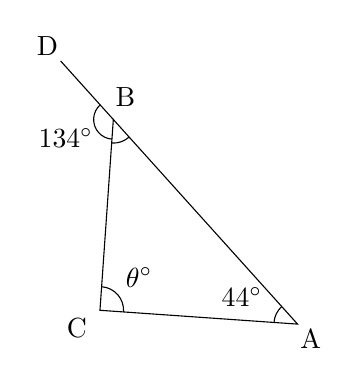
\begin{tikzpicture}[scale=1.0, baseline=(current bounding box.north)]

      \begin{scope}[rotate=132]
        \coordinate (A) at (0,0);
        \coordinate (B) at (3.49681898167051,0);
        \coordinate (D) at (4.4968189816705095,0);
        \coordinate (C) at (intersection cs: first line={(A)--($(A)+(44:4cm)$)}, second line={(B)--($(B)+(180-46:4cm)$)});
        \draw (A) -- (B) -- (C) -- cycle;
        \draw (B) -- (D);

        % Mark angles with arcs
        \draw ($(A)!0.3cm!(B)$) arc [start angle=0, end angle=44, radius=0.3cm];
        \draw ($(B)!0.3cm!(C)$) arc [start angle=180-46, end angle=180, radius=0.3cm];
        \draw ($(C)!0.3cm!(A)$) arc [start angle=180+44, end angle=360-46, radius=0.3cm];
        \draw ($(B)!0.25cm!(D)$) arc [start angle=0, end angle=180-46, radius=0.25cm];

        % Label angles
        \node at ($(A)!-0.25cm!(B)$) {A};
        \node at ($(B)!-0.45cm!(C)!0.2cm!(A)$) {B};
        \node at ($(C)!-0.25cm!(A)!-0.25cm!(B)$) {C};
        \node at ($(D)!-0.25cm!(A)$) {D};

        % Mark angles in degrees
        \coordinate (midBC) at ($(B)!0.5!(C)$);
        \node at ($(A)!0.70cm!(midBC)!0.10cm!(C)$) {$44^\circ$};

        \coordinate (midAC) at ($(A)!0.5!(C)$);
        \node at ($(B)!0.65cm!(midAC)$) {};

        \coordinate (midAB) at ($(A)!0.5!(B)$);
        \node at ($(C)!0.65cm!(midAB)$) {$\theta^\circ$};

        \coordinate (midDC) at ($(D)!0.3!(C)$);
        \node at ($(B)!0.65cm!(midDC)$) {$134^\circ$};


      \end{scope}
    \end{tikzpicture}
\end{minipage}%
\hfill
\begin{minipage}{0.4\textwidth}
  \begin{align*}
    \angle \text{C} &= \angle \text{\dotuline{~~~~~~~}} - \angle \text{\dotuline{~~~~~~~}} \\
    &= \dotuline{~~~~~~~}^\circ  - \dotuline{~~~~~~~}^\circ \\
    &= \dotuline{~~~~~~~}^\circ
  \end{align*}
\end{minipage}
\vspace{1cm} \vfill\begin{minipage}{0.55\textwidth}
  \refstepcounter{minipagecount}
  \noindent{(\theminipagecount)}\quad
  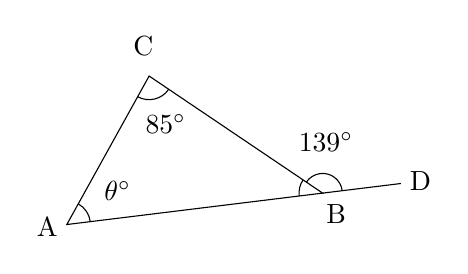
\begin{tikzpicture}[scale=1.0, baseline=(current bounding box.north)]

      \begin{scope}[rotate=7]
        \coordinate (A) at (0,0);
        \coordinate (B) at (3.2734417615540288,0);
        \coordinate (D) at (4.273441761554029,0);
        \coordinate (C) at (intersection cs: first line={(A)--($(A)+(54:4cm)$)}, second line={(B)--($(B)+(180-41:4cm)$)});
        \draw (A) -- (B) -- (C) -- cycle;
        \draw (B) -- (D);

        % Mark angles with arcs
        \draw ($(A)!0.3cm!(B)$) arc [start angle=0, end angle=54, radius=0.3cm];
        \draw ($(B)!0.3cm!(C)$) arc [start angle=180-41, end angle=180, radius=0.3cm];
        \draw ($(C)!0.3cm!(A)$) arc [start angle=180+54, end angle=360-41, radius=0.3cm];
        \draw ($(B)!0.25cm!(D)$) arc [start angle=0, end angle=180-41, radius=0.25cm];

        % Label angles
        \node at ($(A)!-0.25cm!(B)$) {A};
        \node at ($(B)!-0.45cm!(C)!0.2cm!(A)$) {B};
        \node at ($(C)!-0.25cm!(A)!-0.25cm!(B)$) {C};
        \node at ($(D)!-0.25cm!(A)$) {D};

        % Mark angles in degrees
        \coordinate (midBC) at ($(B)!0.5!(C)$);
        \node at ($(A)!0.70cm!(midBC)!0.10cm!(C)$) {$\theta^\circ$};

        \coordinate (midAC) at ($(A)!0.5!(C)$);
        \node at ($(B)!0.65cm!(midAC)$) {};

        \coordinate (midAB) at ($(A)!0.5!(B)$);
        \node at ($(C)!0.65cm!(midAB)$) {$85^\circ$};

        \coordinate (midDC) at ($(D)!0.3!(C)$);
        \node at ($(B)!0.65cm!(midDC)$) {$139^\circ$};


      \end{scope}
    \end{tikzpicture}
\end{minipage}%
\hfill
\begin{minipage}{0.4\textwidth}
  \begin{align*}
    \angle \text{A} &= \angle \text{\dotuline{~~~~~~~}} - \angle \text{\dotuline{~~~~~~~}} \\
    &= \dotuline{~~~~~~~}^\circ  - \dotuline{~~~~~~~}^\circ \\
    &= \dotuline{~~~~~~~}^\circ
  \end{align*}
\end{minipage}
\vspace{1cm} \vfill\begin{minipage}{0.55\textwidth}
  \refstepcounter{minipagecount}
  \noindent{(\theminipagecount)}\quad
  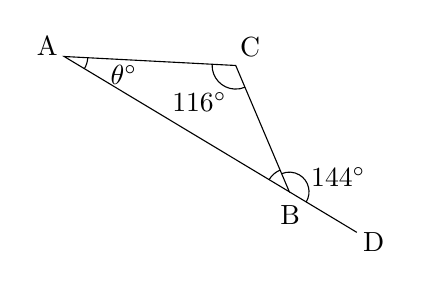
\begin{tikzpicture}[scale=1.0, baseline=(current bounding box.north)]

      \begin{scope}[rotate=329]
        \coordinate (A) at (0,0);
        \coordinate (B) at (3.336474770456516,0);
        \coordinate (D) at (4.336474770456515,0);
        \coordinate (C) at (intersection cs: first line={(A)--($(A)+(28:4cm)$)}, second line={(B)--($(B)+(180-36:4cm)$)});
        \draw (A) -- (B) -- (C) -- cycle;
        \draw (B) -- (D);

        % Mark angles with arcs
        \draw ($(A)!0.3cm!(B)$) arc [start angle=0, end angle=28, radius=0.3cm];
        \draw ($(B)!0.3cm!(C)$) arc [start angle=180-36, end angle=180, radius=0.3cm];
        \draw ($(C)!0.3cm!(A)$) arc [start angle=180+28, end angle=360-36, radius=0.3cm];
        \draw ($(B)!0.25cm!(D)$) arc [start angle=0, end angle=180-36, radius=0.25cm];

        % Label angles
        \node at ($(A)!-0.25cm!(B)$) {A};
        \node at ($(B)!-0.45cm!(C)!0.2cm!(A)$) {B};
        \node at ($(C)!-0.25cm!(A)!-0.25cm!(B)$) {C};
        \node at ($(D)!-0.25cm!(A)$) {D};

        % Mark angles in degrees
        \coordinate (midBC) at ($(B)!0.5!(C)$);
        \node at ($(A)!0.70cm!(midBC)!0.10cm!(C)$) {$\theta^\circ$};

        \coordinate (midAC) at ($(A)!0.5!(C)$);
        \node at ($(B)!0.65cm!(midAC)$) {};

        \coordinate (midAB) at ($(A)!0.5!(B)$);
        \node at ($(C)!0.65cm!(midAB)$) {$116^\circ$};

        \coordinate (midDC) at ($(D)!0.3!(C)$);
        \node at ($(B)!0.65cm!(midDC)$) {$144^\circ$};


      \end{scope}
    \end{tikzpicture}
\end{minipage}%
\hfill
\begin{minipage}{0.4\textwidth}
  \begin{align*}
    \angle \text{A} &= \angle \text{\dotuline{~~~~~~~}} - \angle \text{\dotuline{~~~~~~~}} \\
    &= \dotuline{~~~~~~~}^\circ  - \dotuline{~~~~~~~}^\circ \\
    &= \dotuline{~~~~~~~}^\circ
  \end{align*}
\end{minipage}
\vspace{1cm} \vfill\pagebreak ~ \newline ~ \newline\begin{minipage}{0.55\textwidth}
  \refstepcounter{minipagecount}
  \noindent{(\theminipagecount)}\quad
  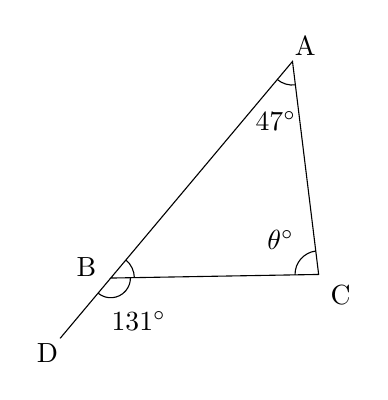
\begin{tikzpicture}[scale=1.0, baseline=(current bounding box.north)]

      \begin{scope}[rotate=230]
        \coordinate (A) at (0,0);
        \coordinate (B) at (3.5912968313361686,0);
        \coordinate (D) at (4.591296831336169,0);
        \coordinate (C) at (intersection cs: first line={(A)--($(A)+(47:4cm)$)}, second line={(B)--($(B)+(180-49:4cm)$)});
        \draw (A) -- (B) -- (C) -- cycle;
        \draw (B) -- (D);

        % Mark angles with arcs
        \draw ($(A)!0.3cm!(B)$) arc [start angle=0, end angle=47, radius=0.3cm];
        \draw ($(B)!0.3cm!(C)$) arc [start angle=180-49, end angle=180, radius=0.3cm];
        \draw ($(C)!0.3cm!(A)$) arc [start angle=180+47, end angle=360-49, radius=0.3cm];
        \draw ($(B)!0.25cm!(D)$) arc [start angle=0, end angle=180-49, radius=0.25cm];

        % Label angles
        \node at ($(A)!-0.25cm!(B)$) {A};
        \node at ($(B)!-0.45cm!(C)!0.2cm!(A)$) {B};
        \node at ($(C)!-0.25cm!(A)!-0.25cm!(B)$) {C};
        \node at ($(D)!-0.25cm!(A)$) {D};

        % Mark angles in degrees
        \coordinate (midBC) at ($(B)!0.5!(C)$);
        \node at ($(A)!0.70cm!(midBC)!0.10cm!(C)$) {$47^\circ$};

        \coordinate (midAC) at ($(A)!0.5!(C)$);
        \node at ($(B)!0.65cm!(midAC)$) {};

        \coordinate (midAB) at ($(A)!0.5!(B)$);
        \node at ($(C)!0.65cm!(midAB)$) {$\theta^\circ$};

        \coordinate (midDC) at ($(D)!0.3!(C)$);
        \node at ($(B)!0.65cm!(midDC)$) {$131^\circ$};


      \end{scope}
    \end{tikzpicture}
\end{minipage}%
\hfill
\begin{minipage}{0.4\textwidth}
  \begin{align*}
    \angle \text{C} &= \angle \text{\dotuline{~~~~~~~}} - \angle \text{\dotuline{~~~~~~~}} \\
    &= \dotuline{~~~~~~~}^\circ  - \dotuline{~~~~~~~}^\circ \\
    &= \dotuline{~~~~~~~}^\circ
  \end{align*}
\end{minipage}
\vspace{1cm} \vfill\begin{minipage}{0.55\textwidth}
  \refstepcounter{minipagecount}
  \noindent{(\theminipagecount)}\quad
  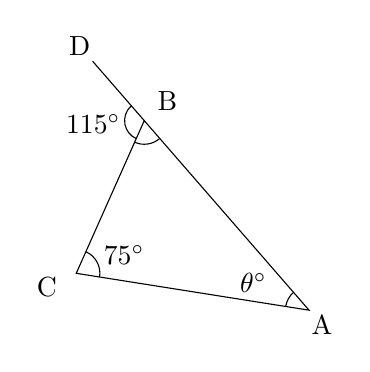
\begin{tikzpicture}[scale=1.0, baseline=(current bounding box.north)]

      \begin{scope}[rotate=131]
        \coordinate (A) at (0,0);
        \coordinate (B) at (3.1893416476160423,0);
        \coordinate (D) at (4.189341647616042,0);
        \coordinate (C) at (intersection cs: first line={(A)--($(A)+(40:4cm)$)}, second line={(B)--($(B)+(180-65:4cm)$)});
        \draw (A) -- (B) -- (C) -- cycle;
        \draw (B) -- (D);

        % Mark angles with arcs
        \draw ($(A)!0.3cm!(B)$) arc [start angle=0, end angle=40, radius=0.3cm];
        \draw ($(B)!0.3cm!(C)$) arc [start angle=180-65, end angle=180, radius=0.3cm];
        \draw ($(C)!0.3cm!(A)$) arc [start angle=180+40, end angle=360-65, radius=0.3cm];
        \draw ($(B)!0.25cm!(D)$) arc [start angle=0, end angle=180-65, radius=0.25cm];

        % Label angles
        \node at ($(A)!-0.25cm!(B)$) {A};
        \node at ($(B)!-0.45cm!(C)!0.2cm!(A)$) {B};
        \node at ($(C)!-0.25cm!(A)!-0.25cm!(B)$) {C};
        \node at ($(D)!-0.25cm!(A)$) {D};

        % Mark angles in degrees
        \coordinate (midBC) at ($(B)!0.5!(C)$);
        \node at ($(A)!0.70cm!(midBC)!0.10cm!(C)$) {$\theta^\circ$};

        \coordinate (midAC) at ($(A)!0.5!(C)$);
        \node at ($(B)!0.65cm!(midAC)$) {};

        \coordinate (midAB) at ($(A)!0.5!(B)$);
        \node at ($(C)!0.65cm!(midAB)$) {$75^\circ$};

        \coordinate (midDC) at ($(D)!0.3!(C)$);
        \node at ($(B)!0.65cm!(midDC)$) {$115^\circ$};


      \end{scope}
    \end{tikzpicture}
\end{minipage}%
\hfill
\begin{minipage}{0.4\textwidth}
  \begin{align*}
    \angle \text{A} &= \angle \text{\dotuline{~~~~~~~}} - \angle \text{\dotuline{~~~~~~~}} \\
    &= \dotuline{~~~~~~~}^\circ  - \dotuline{~~~~~~~}^\circ \\
    &= \dotuline{~~~~~~~}^\circ
  \end{align*}
\end{minipage}
\vspace{1cm} \vfill\begin{minipage}{0.55\textwidth}
  \refstepcounter{minipagecount}
  \noindent{(\theminipagecount)}\quad
  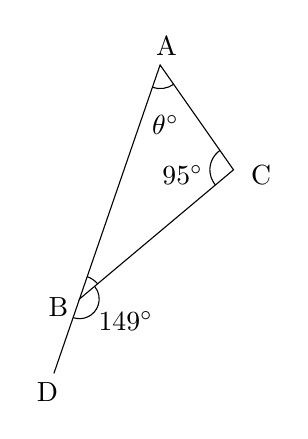
\begin{tikzpicture}[scale=1.0, baseline=(current bounding box.north)]

      \begin{scope}[rotate=251]
        \coordinate (A) at (0,0);
        \coordinate (B) at (3.1433984368842633,0);
        \coordinate (D) at (4.143398436884263,0);
        \coordinate (C) at (intersection cs: first line={(A)--($(A)+(54:4cm)$)}, second line={(B)--($(B)+(180-31:4cm)$)});
        \draw (A) -- (B) -- (C) -- cycle;
        \draw (B) -- (D);

        % Mark angles with arcs
        \draw ($(A)!0.3cm!(B)$) arc [start angle=0, end angle=54, radius=0.3cm];
        \draw ($(B)!0.3cm!(C)$) arc [start angle=180-31, end angle=180, radius=0.3cm];
        \draw ($(C)!0.3cm!(A)$) arc [start angle=180+54, end angle=360-31, radius=0.3cm];
        \draw ($(B)!0.25cm!(D)$) arc [start angle=0, end angle=180-31, radius=0.25cm];

        % Label angles
        \node at ($(A)!-0.25cm!(B)$) {A};
        \node at ($(B)!-0.45cm!(C)!0.2cm!(A)$) {B};
        \node at ($(C)!-0.25cm!(A)!-0.25cm!(B)$) {C};
        \node at ($(D)!-0.25cm!(A)$) {D};

        % Mark angles in degrees
        \coordinate (midBC) at ($(B)!0.5!(C)$);
        \node at ($(A)!0.70cm!(midBC)!0.10cm!(C)$) {$\theta^\circ$};

        \coordinate (midAC) at ($(A)!0.5!(C)$);
        \node at ($(B)!0.65cm!(midAC)$) {};

        \coordinate (midAB) at ($(A)!0.5!(B)$);
        \node at ($(C)!0.65cm!(midAB)$) {$95^\circ$};

        \coordinate (midDC) at ($(D)!0.3!(C)$);
        \node at ($(B)!0.65cm!(midDC)$) {$149^\circ$};


      \end{scope}
    \end{tikzpicture}
\end{minipage}%
\hfill
\begin{minipage}{0.4\textwidth}
  \begin{align*}
    \angle \text{A} &= \angle \text{\dotuline{~~~~~~~}} - \angle \text{\dotuline{~~~~~~~}} \\
    &= \dotuline{~~~~~~~}^\circ  - \dotuline{~~~~~~~}^\circ \\
    &= \dotuline{~~~~~~~}^\circ
  \end{align*}
\end{minipage}
\vspace{1cm} \vfill\begin{minipage}{0.55\textwidth}
  \refstepcounter{minipagecount}
  \noindent{(\theminipagecount)}\quad
  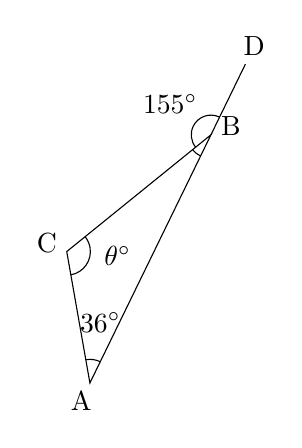
\begin{tikzpicture}[scale=1.0, baseline=(current bounding box.north)]

      \begin{scope}[rotate=64]
        \coordinate (A) at (0,0);
        \coordinate (B) at (3.506499148502966,0);
        \coordinate (D) at (4.506499148502966,0);
        \coordinate (C) at (intersection cs: first line={(A)--($(A)+(36:4cm)$)}, second line={(B)--($(B)+(180-25:4cm)$)});
        \draw (A) -- (B) -- (C) -- cycle;
        \draw (B) -- (D);

        % Mark angles with arcs
        \draw ($(A)!0.3cm!(B)$) arc [start angle=0, end angle=36, radius=0.3cm];
        \draw ($(B)!0.3cm!(C)$) arc [start angle=180-25, end angle=180, radius=0.3cm];
        \draw ($(C)!0.3cm!(A)$) arc [start angle=180+36, end angle=360-25, radius=0.3cm];
        \draw ($(B)!0.25cm!(D)$) arc [start angle=0, end angle=180-25, radius=0.25cm];

        % Label angles
        \node at ($(A)!-0.25cm!(B)$) {A};
        \node at ($(B)!-0.45cm!(C)!0.2cm!(A)$) {B};
        \node at ($(C)!-0.25cm!(A)!-0.25cm!(B)$) {C};
        \node at ($(D)!-0.25cm!(A)$) {D};

        % Mark angles in degrees
        \coordinate (midBC) at ($(B)!0.5!(C)$);
        \node at ($(A)!0.70cm!(midBC)!0.10cm!(C)$) {$36^\circ$};

        \coordinate (midAC) at ($(A)!0.5!(C)$);
        \node at ($(B)!0.65cm!(midAC)$) {};

        \coordinate (midAB) at ($(A)!0.5!(B)$);
        \node at ($(C)!0.65cm!(midAB)$) {$\theta^\circ$};

        \coordinate (midDC) at ($(D)!0.3!(C)$);
        \node at ($(B)!0.65cm!(midDC)$) {$155^\circ$};


      \end{scope}
    \end{tikzpicture}
\end{minipage}%
\hfill
\begin{minipage}{0.4\textwidth}
  \begin{align*}
    \angle \text{C} &= \angle \text{\dotuline{~~~~~~~}} - \angle \text{\dotuline{~~~~~~~}} \\
    &= \dotuline{~~~~~~~}^\circ  - \dotuline{~~~~~~~}^\circ \\
    &= \dotuline{~~~~~~~}^\circ
  \end{align*}
\end{minipage}
\vspace{1cm} \vfill\pagebreak ~ \newline ~ \newline\begin{minipage}{0.55\textwidth}
  \refstepcounter{minipagecount}
  \noindent{(\theminipagecount)}\quad
  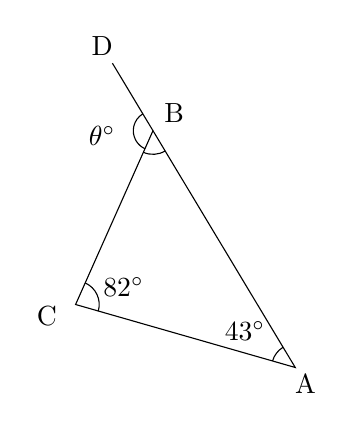
\begin{tikzpicture}[scale=1.0, baseline=(current bounding box.north)]

      \begin{scope}[rotate=121]
        \coordinate (A) at (0,0);
        \coordinate (B) at (3.5079339949307338,0);
        \coordinate (D) at (4.507933994930734,0);
        \coordinate (C) at (intersection cs: first line={(A)--($(A)+(43:4cm)$)}, second line={(B)--($(B)+(180-55:4cm)$)});
        \draw (A) -- (B) -- (C) -- cycle;
        \draw (B) -- (D);

        % Mark angles with arcs
        \draw ($(A)!0.3cm!(B)$) arc [start angle=0, end angle=43, radius=0.3cm];
        \draw ($(B)!0.3cm!(C)$) arc [start angle=180-55, end angle=180, radius=0.3cm];
        \draw ($(C)!0.3cm!(A)$) arc [start angle=180+43, end angle=360-55, radius=0.3cm];
        \draw ($(B)!0.25cm!(D)$) arc [start angle=0, end angle=180-55, radius=0.25cm];

        % Label angles
        \node at ($(A)!-0.25cm!(B)$) {A};
        \node at ($(B)!-0.45cm!(C)!0.2cm!(A)$) {B};
        \node at ($(C)!-0.25cm!(A)!-0.25cm!(B)$) {C};
        \node at ($(D)!-0.25cm!(A)$) {D};

        % Mark angles in degrees
        \coordinate (midBC) at ($(B)!0.5!(C)$);
        \node at ($(A)!0.70cm!(midBC)!0.10cm!(C)$) {$43^\circ$};

        \coordinate (midAC) at ($(A)!0.5!(C)$);
        \node at ($(B)!0.65cm!(midAC)$) {};

        \coordinate (midAB) at ($(A)!0.5!(B)$);
        \node at ($(C)!0.65cm!(midAB)$) {$82^\circ$};

        \coordinate (midDC) at ($(D)!0.3!(C)$);
        \node at ($(B)!0.65cm!(midDC)$) {$\theta^\circ$};


      \end{scope}
    \end{tikzpicture}
\end{minipage}%
\hfill
\begin{minipage}{0.4\textwidth}
  \begin{align*}
    \angle \text{DBC} &= \angle \text{\dotuline{~~~~~~~}} + \angle \text{\dotuline{~~~~~~~}} \\
    &= \dotuline{~~~~~~~}^\circ  + \dotuline{~~~~~~~}^\circ \\
    &= \dotuline{~~~~~~~}^\circ
  \end{align*}
\end{minipage}
\vspace{1cm} \vfill\begin{minipage}{0.55\textwidth}
  \refstepcounter{minipagecount}
  \noindent{(\theminipagecount)}\quad
  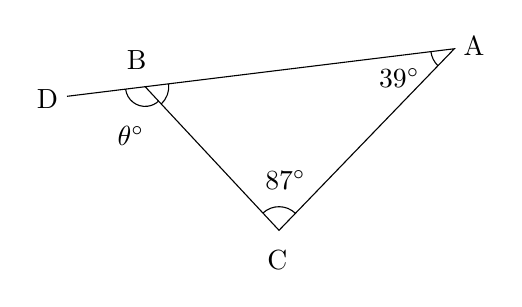
\begin{tikzpicture}[scale=1.0, baseline=(current bounding box.north)]

      \begin{scope}[rotate=187]
        \coordinate (A) at (0,0);
        \coordinate (B) at (3.9562286920063627,0);
        \coordinate (D) at (4.956228692006363,0);
        \coordinate (C) at (intersection cs: first line={(A)--($(A)+(39:4cm)$)}, second line={(B)--($(B)+(180-54:4cm)$)});
        \draw (A) -- (B) -- (C) -- cycle;
        \draw (B) -- (D);

        % Mark angles with arcs
        \draw ($(A)!0.3cm!(B)$) arc [start angle=0, end angle=39, radius=0.3cm];
        \draw ($(B)!0.3cm!(C)$) arc [start angle=180-54, end angle=180, radius=0.3cm];
        \draw ($(C)!0.3cm!(A)$) arc [start angle=180+39, end angle=360-54, radius=0.3cm];
        \draw ($(B)!0.25cm!(D)$) arc [start angle=0, end angle=180-54, radius=0.25cm];

        % Label angles
        \node at ($(A)!-0.25cm!(B)$) {A};
        \node at ($(B)!-0.45cm!(C)!0.2cm!(A)$) {B};
        \node at ($(C)!-0.25cm!(A)!-0.25cm!(B)$) {C};
        \node at ($(D)!-0.25cm!(A)$) {D};

        % Mark angles in degrees
        \coordinate (midBC) at ($(B)!0.5!(C)$);
        \node at ($(A)!0.70cm!(midBC)!0.10cm!(C)$) {$39^\circ$};

        \coordinate (midAC) at ($(A)!0.5!(C)$);
        \node at ($(B)!0.65cm!(midAC)$) {};

        \coordinate (midAB) at ($(A)!0.5!(B)$);
        \node at ($(C)!0.65cm!(midAB)$) {$87^\circ$};

        \coordinate (midDC) at ($(D)!0.3!(C)$);
        \node at ($(B)!0.65cm!(midDC)$) {$\theta^\circ$};


      \end{scope}
    \end{tikzpicture}
\end{minipage}%
\hfill
\begin{minipage}{0.4\textwidth}
  \begin{align*}
    \angle \text{DBC} &= \angle \text{\dotuline{~~~~~~~}} + \angle \text{\dotuline{~~~~~~~}} \\
    &= \dotuline{~~~~~~~}^\circ  + \dotuline{~~~~~~~}^\circ \\
    &= \dotuline{~~~~~~~}^\circ
  \end{align*}
\end{minipage}
\vspace{1cm} \vfill\begin{minipage}{0.55\textwidth}
  \refstepcounter{minipagecount}
  \noindent{(\theminipagecount)}\quad
  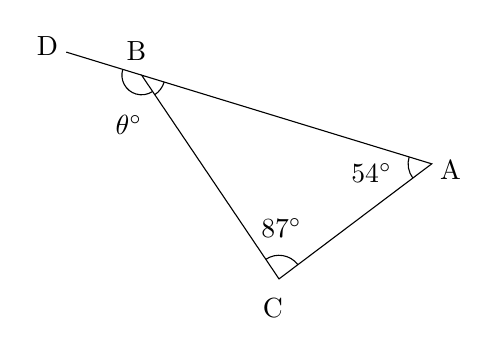
\begin{tikzpicture}[scale=1.0, baseline=(current bounding box.north)]

      \begin{scope}[rotate=163]
        \coordinate (A) at (0,0);
        \coordinate (B) at (3.8531373513610365,0);
        \coordinate (D) at (4.8531373513610365,0);
        \coordinate (C) at (intersection cs: first line={(A)--($(A)+(54:4cm)$)}, second line={(B)--($(B)+(180-39:4cm)$)});
        \draw (A) -- (B) -- (C) -- cycle;
        \draw (B) -- (D);

        % Mark angles with arcs
        \draw ($(A)!0.3cm!(B)$) arc [start angle=0, end angle=54, radius=0.3cm];
        \draw ($(B)!0.3cm!(C)$) arc [start angle=180-39, end angle=180, radius=0.3cm];
        \draw ($(C)!0.3cm!(A)$) arc [start angle=180+54, end angle=360-39, radius=0.3cm];
        \draw ($(B)!0.25cm!(D)$) arc [start angle=0, end angle=180-39, radius=0.25cm];

        % Label angles
        \node at ($(A)!-0.25cm!(B)$) {A};
        \node at ($(B)!-0.45cm!(C)!0.2cm!(A)$) {B};
        \node at ($(C)!-0.25cm!(A)!-0.25cm!(B)$) {C};
        \node at ($(D)!-0.25cm!(A)$) {D};

        % Mark angles in degrees
        \coordinate (midBC) at ($(B)!0.5!(C)$);
        \node at ($(A)!0.70cm!(midBC)!0.10cm!(C)$) {$54^\circ$};

        \coordinate (midAC) at ($(A)!0.5!(C)$);
        \node at ($(B)!0.65cm!(midAC)$) {};

        \coordinate (midAB) at ($(A)!0.5!(B)$);
        \node at ($(C)!0.65cm!(midAB)$) {$87^\circ$};

        \coordinate (midDC) at ($(D)!0.3!(C)$);
        \node at ($(B)!0.65cm!(midDC)$) {$\theta^\circ$};


      \end{scope}
    \end{tikzpicture}
\end{minipage}%
\hfill
\begin{minipage}{0.4\textwidth}
  \begin{align*}
    \angle \text{DBC} &= \angle \text{\dotuline{~~~~~~~}} + \angle \text{\dotuline{~~~~~~~}} \\
    &= \dotuline{~~~~~~~}^\circ  + \dotuline{~~~~~~~}^\circ \\
    &= \dotuline{~~~~~~~}^\circ
  \end{align*}
\end{minipage}
\vspace{1cm} \vfill\begin{minipage}{0.55\textwidth}
  \refstepcounter{minipagecount}
  \noindent{(\theminipagecount)}\quad
  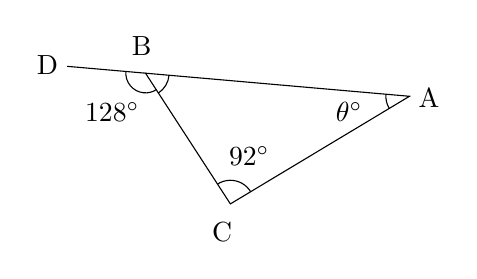
\begin{tikzpicture}[scale=1.0, baseline=(current bounding box.north)]

      \begin{scope}[rotate=175]
        \coordinate (A) at (0,0);
        \coordinate (B) at (3.365326368370563,0);
        \coordinate (D) at (4.365326368370563,0);
        \coordinate (C) at (intersection cs: first line={(A)--($(A)+(36:4cm)$)}, second line={(B)--($(B)+(180-52:4cm)$)});
        \draw (A) -- (B) -- (C) -- cycle;
        \draw (B) -- (D);

        % Mark angles with arcs
        \draw ($(A)!0.3cm!(B)$) arc [start angle=0, end angle=36, radius=0.3cm];
        \draw ($(B)!0.3cm!(C)$) arc [start angle=180-52, end angle=180, radius=0.3cm];
        \draw ($(C)!0.3cm!(A)$) arc [start angle=180+36, end angle=360-52, radius=0.3cm];
        \draw ($(B)!0.25cm!(D)$) arc [start angle=0, end angle=180-52, radius=0.25cm];

        % Label angles
        \node at ($(A)!-0.25cm!(B)$) {A};
        \node at ($(B)!-0.45cm!(C)!0.2cm!(A)$) {B};
        \node at ($(C)!-0.25cm!(A)!-0.25cm!(B)$) {C};
        \node at ($(D)!-0.25cm!(A)$) {D};

        % Mark angles in degrees
        \coordinate (midBC) at ($(B)!0.5!(C)$);
        \node at ($(A)!0.70cm!(midBC)!0.10cm!(C)$) {$\theta^\circ$};

        \coordinate (midAC) at ($(A)!0.5!(C)$);
        \node at ($(B)!0.65cm!(midAC)$) {};

        \coordinate (midAB) at ($(A)!0.5!(B)$);
        \node at ($(C)!0.65cm!(midAB)$) {$92^\circ$};

        \coordinate (midDC) at ($(D)!0.3!(C)$);
        \node at ($(B)!0.65cm!(midDC)$) {$128^\circ$};


      \end{scope}
    \end{tikzpicture}
\end{minipage}%
\hfill
\begin{minipage}{0.4\textwidth}
  \begin{align*}
    \angle \text{A} &= \angle \text{\dotuline{~~~~~~~}} - \angle \text{\dotuline{~~~~~~~}} \\
    &= \dotuline{~~~~~~~}^\circ  - \dotuline{~~~~~~~}^\circ \\
    &= \dotuline{~~~~~~~}^\circ
  \end{align*}
\end{minipage}
\vspace{1cm} \vfill\pagebreak ~ \newline ~ \newline\begin{minipage}{0.55\textwidth}
  \refstepcounter{minipagecount}
  \noindent{(\theminipagecount)}\quad
  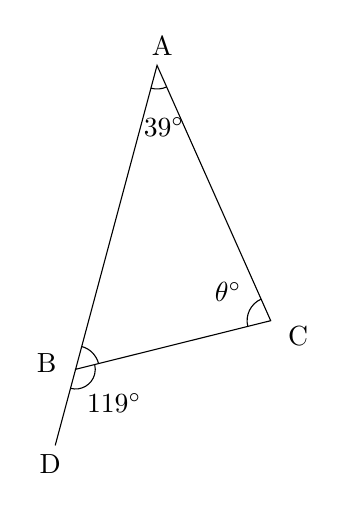
\begin{tikzpicture}[scale=1.0, baseline=(current bounding box.north)]

      \begin{scope}[rotate=255]
        \coordinate (A) at (0,0);
        \coordinate (B) at (3.996112485915069,0);
        \coordinate (D) at (4.996112485915069,0);
        \coordinate (C) at (intersection cs: first line={(A)--($(A)+(39:4cm)$)}, second line={(B)--($(B)+(180-61:4cm)$)});
        \draw (A) -- (B) -- (C) -- cycle;
        \draw (B) -- (D);

        % Mark angles with arcs
        \draw ($(A)!0.3cm!(B)$) arc [start angle=0, end angle=39, radius=0.3cm];
        \draw ($(B)!0.3cm!(C)$) arc [start angle=180-61, end angle=180, radius=0.3cm];
        \draw ($(C)!0.3cm!(A)$) arc [start angle=180+39, end angle=360-61, radius=0.3cm];
        \draw ($(B)!0.25cm!(D)$) arc [start angle=0, end angle=180-61, radius=0.25cm];

        % Label angles
        \node at ($(A)!-0.25cm!(B)$) {A};
        \node at ($(B)!-0.45cm!(C)!0.2cm!(A)$) {B};
        \node at ($(C)!-0.25cm!(A)!-0.25cm!(B)$) {C};
        \node at ($(D)!-0.25cm!(A)$) {D};

        % Mark angles in degrees
        \coordinate (midBC) at ($(B)!0.5!(C)$);
        \node at ($(A)!0.70cm!(midBC)!0.10cm!(C)$) {$39^\circ$};

        \coordinate (midAC) at ($(A)!0.5!(C)$);
        \node at ($(B)!0.65cm!(midAC)$) {};

        \coordinate (midAB) at ($(A)!0.5!(B)$);
        \node at ($(C)!0.65cm!(midAB)$) {$\theta^\circ$};

        \coordinate (midDC) at ($(D)!0.3!(C)$);
        \node at ($(B)!0.65cm!(midDC)$) {$119^\circ$};


      \end{scope}
    \end{tikzpicture}
\end{minipage}%
\hfill
\begin{minipage}{0.4\textwidth}
  \begin{align*}
    \angle \text{C} &= \angle \text{\dotuline{~~~~~~~}} - \angle \text{\dotuline{~~~~~~~}} \\
    &= \dotuline{~~~~~~~}^\circ  - \dotuline{~~~~~~~}^\circ \\
    &= \dotuline{~~~~~~~}^\circ
  \end{align*}
\end{minipage}
\vspace{1cm} \vfill\begin{minipage}{0.55\textwidth}
  \refstepcounter{minipagecount}
  \noindent{(\theminipagecount)}\quad
  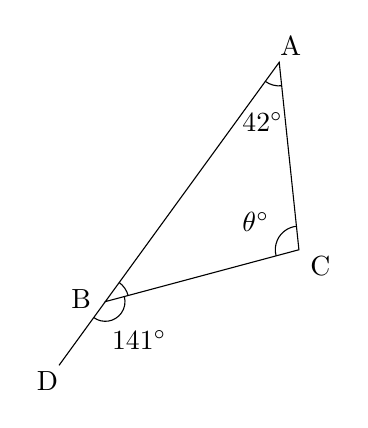
\begin{tikzpicture}[scale=1.0, baseline=(current bounding box.north)]

      \begin{scope}[rotate=234]
        \coordinate (A) at (0,0);
        \coordinate (B) at (3.7572385892626583,0);
        \coordinate (D) at (4.757238589262658,0);
        \coordinate (C) at (intersection cs: first line={(A)--($(A)+(42:4cm)$)}, second line={(B)--($(B)+(180-39:4cm)$)});
        \draw (A) -- (B) -- (C) -- cycle;
        \draw (B) -- (D);

        % Mark angles with arcs
        \draw ($(A)!0.3cm!(B)$) arc [start angle=0, end angle=42, radius=0.3cm];
        \draw ($(B)!0.3cm!(C)$) arc [start angle=180-39, end angle=180, radius=0.3cm];
        \draw ($(C)!0.3cm!(A)$) arc [start angle=180+42, end angle=360-39, radius=0.3cm];
        \draw ($(B)!0.25cm!(D)$) arc [start angle=0, end angle=180-39, radius=0.25cm];

        % Label angles
        \node at ($(A)!-0.25cm!(B)$) {A};
        \node at ($(B)!-0.45cm!(C)!0.2cm!(A)$) {B};
        \node at ($(C)!-0.25cm!(A)!-0.25cm!(B)$) {C};
        \node at ($(D)!-0.25cm!(A)$) {D};

        % Mark angles in degrees
        \coordinate (midBC) at ($(B)!0.5!(C)$);
        \node at ($(A)!0.70cm!(midBC)!0.10cm!(C)$) {$42^\circ$};

        \coordinate (midAC) at ($(A)!0.5!(C)$);
        \node at ($(B)!0.65cm!(midAC)$) {};

        \coordinate (midAB) at ($(A)!0.5!(B)$);
        \node at ($(C)!0.65cm!(midAB)$) {$\theta^\circ$};

        \coordinate (midDC) at ($(D)!0.3!(C)$);
        \node at ($(B)!0.65cm!(midDC)$) {$141^\circ$};


      \end{scope}
    \end{tikzpicture}
\end{minipage}%
\hfill
\begin{minipage}{0.4\textwidth}
  \begin{align*}
    \angle \text{C} &= \angle \text{\dotuline{~~~~~~~}} - \angle \text{\dotuline{~~~~~~~}} \\
    &= \dotuline{~~~~~~~}^\circ  - \dotuline{~~~~~~~}^\circ \\
    &= \dotuline{~~~~~~~}^\circ
  \end{align*}
\end{minipage}
\vspace{1cm} \vfill\begin{minipage}{0.55\textwidth}
  \refstepcounter{minipagecount}
  \noindent{(\theminipagecount)}\quad
  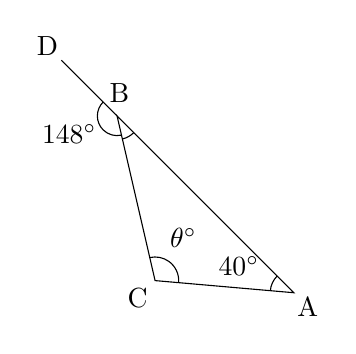
\begin{tikzpicture}[scale=1.0, baseline=(current bounding box.north)]

      \begin{scope}[rotate=135]
        \coordinate (A) at (0,0);
        \coordinate (B) at (3.175177503439901,0);
        \coordinate (D) at (4.175177503439901,0);
        \coordinate (C) at (intersection cs: first line={(A)--($(A)+(40:4cm)$)}, second line={(B)--($(B)+(180-32:4cm)$)});
        \draw (A) -- (B) -- (C) -- cycle;
        \draw (B) -- (D);

        % Mark angles with arcs
        \draw ($(A)!0.3cm!(B)$) arc [start angle=0, end angle=40, radius=0.3cm];
        \draw ($(B)!0.3cm!(C)$) arc [start angle=180-32, end angle=180, radius=0.3cm];
        \draw ($(C)!0.3cm!(A)$) arc [start angle=180+40, end angle=360-32, radius=0.3cm];
        \draw ($(B)!0.25cm!(D)$) arc [start angle=0, end angle=180-32, radius=0.25cm];

        % Label angles
        \node at ($(A)!-0.25cm!(B)$) {A};
        \node at ($(B)!-0.45cm!(C)!0.2cm!(A)$) {B};
        \node at ($(C)!-0.25cm!(A)!-0.25cm!(B)$) {C};
        \node at ($(D)!-0.25cm!(A)$) {D};

        % Mark angles in degrees
        \coordinate (midBC) at ($(B)!0.5!(C)$);
        \node at ($(A)!0.70cm!(midBC)!0.10cm!(C)$) {$40^\circ$};

        \coordinate (midAC) at ($(A)!0.5!(C)$);
        \node at ($(B)!0.65cm!(midAC)$) {};

        \coordinate (midAB) at ($(A)!0.5!(B)$);
        \node at ($(C)!0.65cm!(midAB)$) {$\theta^\circ$};

        \coordinate (midDC) at ($(D)!0.3!(C)$);
        \node at ($(B)!0.65cm!(midDC)$) {$148^\circ$};


      \end{scope}
    \end{tikzpicture}
\end{minipage}%
\hfill
\begin{minipage}{0.4\textwidth}
  \begin{align*}
    \angle \text{C} &= \angle \text{\dotuline{~~~~~~~}} - \angle \text{\dotuline{~~~~~~~}} \\
    &= \dotuline{~~~~~~~}^\circ  - \dotuline{~~~~~~~}^\circ \\
    &= \dotuline{~~~~~~~}^\circ
  \end{align*}
\end{minipage}
\vspace{1cm} \vfill\begin{minipage}{0.55\textwidth}
  \refstepcounter{minipagecount}
  \noindent{(\theminipagecount)}\quad
  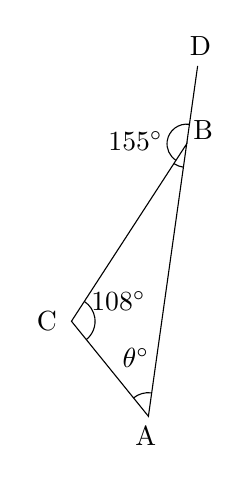
\begin{tikzpicture}[scale=1.0, baseline=(current bounding box.north)]

      \begin{scope}[rotate=82]
        \coordinate (A) at (0,0);
        \coordinate (B) at (3.4943098487047615,0);
        \coordinate (D) at (4.494309848704761,0);
        \coordinate (C) at (intersection cs: first line={(A)--($(A)+(47:4cm)$)}, second line={(B)--($(B)+(180-25:4cm)$)});
        \draw (A) -- (B) -- (C) -- cycle;
        \draw (B) -- (D);

        % Mark angles with arcs
        \draw ($(A)!0.3cm!(B)$) arc [start angle=0, end angle=47, radius=0.3cm];
        \draw ($(B)!0.3cm!(C)$) arc [start angle=180-25, end angle=180, radius=0.3cm];
        \draw ($(C)!0.3cm!(A)$) arc [start angle=180+47, end angle=360-25, radius=0.3cm];
        \draw ($(B)!0.25cm!(D)$) arc [start angle=0, end angle=180-25, radius=0.25cm];

        % Label angles
        \node at ($(A)!-0.25cm!(B)$) {A};
        \node at ($(B)!-0.45cm!(C)!0.2cm!(A)$) {B};
        \node at ($(C)!-0.25cm!(A)!-0.25cm!(B)$) {C};
        \node at ($(D)!-0.25cm!(A)$) {D};

        % Mark angles in degrees
        \coordinate (midBC) at ($(B)!0.5!(C)$);
        \node at ($(A)!0.70cm!(midBC)!0.10cm!(C)$) {$\theta^\circ$};

        \coordinate (midAC) at ($(A)!0.5!(C)$);
        \node at ($(B)!0.65cm!(midAC)$) {};

        \coordinate (midAB) at ($(A)!0.5!(B)$);
        \node at ($(C)!0.65cm!(midAB)$) {$108^\circ$};

        \coordinate (midDC) at ($(D)!0.3!(C)$);
        \node at ($(B)!0.65cm!(midDC)$) {$155^\circ$};


      \end{scope}
    \end{tikzpicture}
\end{minipage}%
\hfill
\begin{minipage}{0.4\textwidth}
  \begin{align*}
    \angle \text{A} &= \angle \text{\dotuline{~~~~~~~}} - \angle \text{\dotuline{~~~~~~~}} \\
    &= \dotuline{~~~~~~~}^\circ  - \dotuline{~~~~~~~}^\circ \\
    &= \dotuline{~~~~~~~}^\circ
  \end{align*}
\end{minipage}
\vspace{1cm} \vfill

\end{document}
